\documentclass[10pt,twocolumn,letterpaper]{article}
\usepackage[margin=0.75in,columnsep=0.25in]{geometry}
\usepackage[T1]{fontenc}
\usepackage[utf8]{inputenc}
\usepackage{lmodern}
\usepackage{microtype}
\usepackage{amsmath}
\usepackage{graphicx}
\usepackage{booktabs}
\usepackage{caption}
\usepackage{xurl}
\usepackage[hidelinks,breaklinks]{hyperref}
\usepackage{placeins}
\captionsetup{font=small,labelfont=bf,skip=5pt}
\graphicspath{{figures/}}
\setlength{\textfloatsep}{10pt plus 2pt minus 2pt}
\setlength{\dbltextfloatsep}{12pt plus 2pt minus 2pt}
\setlength{\floatsep}{9pt plus 2pt minus 2pt}
\setlength{\emergencystretch}{1em}
\renewcommand{\topfraction}{0.95}
\renewcommand{\dbltopfraction}{0.95}
\renewcommand{\textfraction}{0.05}
\renewcommand{\floatpagefraction}{0.8}
\renewcommand{\dblfloatpagefraction}{0.8}
\hypersetup{pdftitle={Byte-compatible fused KV-cache handoff: separating quality evidence from implementation cost},pdfauthor={Jie Chen and Sheng Wei}}
\title{Byte-compatible fused KV-cache handoff:\\separating quality evidence from implementation cost}
\author{Jie Chen \and Sheng Wei}
\date{}
\begin{document}
\raggedbottom
\makeatletter
\twocolumn[\begin{@twocolumnfalse}
\maketitle
\begin{abstract}
Quantizing a KV cache reduces communication but adds encoding, reconstruction
and allocation work. We distinguish these costs using two implementations of
the same cache representation. The original reference study evaluated
Qwen3-4B-Instruct-2507 on 900 unique RULER prompts, seven conditions and real
GPU RDMA. All 6,300 predictions recovered every target, while conservative
simultaneous bounds left the proposed two-percentage-point preservation margin
inconclusive. INT8 and INT4 reduced application bytes, but the reference
PyTorch implementation made quantized handoff slower than BF16. We introduce
an optional Triton implementation that writes directly into the final frame
and constructs a fresh receiver cache without redundant full-cache copies.
An actual-model microbenchmark verified complete packet and reconstructed
cache equality across 27 prompt/precision cells. At the 16K budget, descriptive
codec-only encode-plus-decode summaries fell from 71.58 to 6.99\,ms for INT8 and
104.52 to 17.30\,ms for INT4. A matched three-block native-RDMA pilot completed
378 predictions on nine unique prompts with exact cross-backend token equality.
At 16K, fused INT8 and INT4 median handoffs were 49.03 and 43.62\,ms, versus
124.11 and 144.28\,ms for the matching reference backend and 79.76\,ms for fused
BF16. These descriptive pilot measurements reverse the reference's median
precision ordering. The optional-backend results are exploratory measurements
on nine unique pilot prompts, not a rerun of the 900-prompt quality experiment
or proof of population preservation. The revised evidence separates a valid
reference-backend result from the implementation choices that shape complete
handoff latency.
\end{abstract}
\vspace{8pt}
\end{@twocolumnfalse}]
\makeatother

\section{Introduction}
Disaggregated inference transfers the prompt's KV cache from a prefill worker
to a decode worker. A compressed representation can reduce communication while
increasing the time needed to prepare and reconstruct that cache. The relevant
quantity is the complete handoff, alongside downstream quality and memory cost.

Our original experiment found that BF16 transfer was faster than INT8 or packed
INT4 on an H200 fabric when using a transparent PyTorch codec. That observation
describes a particular implementation. It does not establish that cache
compression is inherently slower on this hardware. We evaluate a byte-compatible
alternative that removes intermediate tensor operations, packing concatenations
and redundant receiver copies while leaving the model, quantization rules and
transport policy fixed.

fabric-lib supplies one-sided GPU communication and immediate notifications
for disaggregated LLM systems~\cite{fabric}. RULER provides controlled
long-context retrieval tasks~\cite{ruler}. KIVI motivates different quantization
axes for keys and values~\cite{kivi}; our group-32 INT4 handoff codec is a
separate implementation, not a reproduction of its complete two-bit inference
system. We use the official Qwen3-4B-Instruct-2507 model and
tokenizer~\cite{qwen}. Our contribution is a controlled implementation
comparison with explicit quality, byte, ownership and timing boundaries,
rather than a new quantization algorithm.

\section{Shared model, representation and handoff protocol}
\subsection{Model and continuation}
Both implementations use Qwen/Qwen3-4B-Instruct-2507 with identical BF16 weights
and tokenizer, SDPA attention, batch size one and greedy decoding. Model and
input-source revisions are pinned (Appendix~\ref{sec:repro}). Newly generated
KV remains BF16. The sender prefills the complete document and question and
chooses the first output token from its final prompt logits. The receiver
receives that choice and generates subsequent tokens using the reconstructed
cache. Quantization therefore cannot change the first output token in this
protocol. This boundary is common to all conditions and limits conclusions
about sensitivity at the prompt/output transition.

The seven conditions are local BF16, local INT8 and INT4 reconstruction,
BF16/INT8/INT4 native transfer, and text transfer with receiver prefill. Each
continuation uses a fresh cache. Exact local/remote token-ID comparisons test
the transfer path independently of quantized-versus-BF16 quality comparisons.

\subsection{Identical cache format and native transport}
Both backends implement the same packed frame format. INT8 uses symmetric
per-head/token quantization. INT4 uses asymmetric group-32 quantization,
grouping K along tokens and V along channels, with FP16 scales and offsets.
Two four-bit values are physically packed into each byte. Padding and
quantization parameters are part of the actual encoded buffer; canonical JSON
describes its sections.

For input length $S$, raw BF16 storage is $147{,}456S$ bytes. Ignoring JSON and
partial-group padding, INT8 and INT4 require 74,880 and 46,080 bytes/token,
respectively: 50.78125\% and 31.25\% of BF16. These are format calculations,
not network measurements. Metadata prevents a fourfold end-to-end reduction
for INT4. Actual application bytes also include control framing up to readiness.

Both backends use the same native Rust endpoint and pinned fabric-lib
transport. GPU/NIC selection follows PCI proximity, NUMA and scheduler CPU
affinity. Data writes are bounded at 256\,MiB, with the receiver immediate on
the final write. The validated allocator setting disables expandable segments.
Source and sink registration remain \emph{per handoff/request}: each whole
frame is registered once, rather than once per bounded write. The optional
backend does not introduce a registration pool, network pacing or pipelining.
Cache payload transfer stays on GPU RDMA without a host-staging fallback.

\subsection{Measurement boundary}
Encoding, transfer and reconstruction are sequential. A sender monotonic timer
runs from cache-ready through receipt of a receiver-ready ACK. It includes
encoding, control framing, dynamic registration, allocation, transport,
reconstruction, synchronization and the return ACK. Readiness means a fresh
\texttt{DynamicCache} is available for model execution. The common continuation
helper then makes its private cache copy before decoding; that copy and
generation remain outside the handoff interval. This measures cache readiness
rather than time to the first receiver decoding step. Model loading and
endpoint setup are startup costs. No timing subtraction crosses hosts.

Codec stage measurements synchronize CUDA around host wall-clock timers and
include dispatch, allocation, validation and cache construction. They are not
kernel-only CUDA-event timings. Encoded size and application-frame bytes are
separate from physical link traffic: network headers and unobserved provider
connection traffic are excluded, and prediction responses are post-ACK bytes.

Handoff memory records allocator baselines and peak allocation above those
baselines. Receiver peaks include reconstructed-cache residency, not only
transient workspace. Native registration borrows storage; registered bytes do
not represent a separate copy. Driver/provider allocations are not inferred
from PyTorch statistics.

\section{Optional fused implementation}
\subsection{Direct encoding and fresh-cache reconstruction}
The explicitly selected fused backend allocates one final byte frame. A fused
kernel for each K or V tensor reads its strides, computes the selected
quantization and writes codes and FP16 parameters into the assigned section.
It avoids intermediate floating-point tensors, separate packing buffers and a
final full-frame concatenation. Quantized-cache validation accumulates into
one device error flag, read once per cache. The raw codec has a linear path
for contiguous inputs and a stride-aware path otherwise.

Decode writes each reconstructed tensor into fresh storage. In pinned
Transformers 4.56.2, \texttt{DynamicCache.update} and its data constructor
concatenate an empty tensor with incoming cache data, creating another copy.
The fused backend gives already-owned outputs to fresh \texttt{DynamicLayer}
objects directly. The resulting cache aliases neither the received frame nor
the sender's cache, and supports subsequent ordinary cache updates. The
comparison therefore covers fused tensor operations \emph{and cache-construction/
allocation changes}; it is not an isolated attribution to a single GPU kernel.

The backend remains optional; the PyTorch implementation is the default.
Peers negotiate and record backend identity, reject mismatches and reject
backend changes during resume. The fused path requires CUDA and does not
silently substitute the reference implementation.

\subsection{Numerical compatibility and compilation}
The implementation preserves edge padding, low-nibble-first packing, FP16
parameter rounding and ties-to-even quantization. FP32 scalar reciprocal
multiplication follows the reference scale computation; quantization uses
correctly rounded division. Decode multiplication and addition remain separate
to prevent fused multiply-add from changing reconstructed bits. Byte-level
parameter accesses support unaligned metadata sections.

Prompt lengths, strides, section offsets and group counts remain runtime kernel
arguments. Codec/layout choices are specialized without specializing each
prompt length. Every selected prompt and condition is warmed before paired
measurement. The standalone codec benchmark also monitors Triton JIT activity
and rejects measured compilation or cache-loading events.

\section{Evaluation design and statistical scope}
\subsection{Retrieval population and distinct experiment strata}
The RULER tasks are \texttt{niah\_single\_2}, requesting one numeric value for a
word key; \texttt{niah\_multikey\_1}, requesting one value among four key/value
facts; and \texttt{niah\_multiquery}, requesting all four values. All use the
official essay haystack. This subset does not cover the full RULER benchmark.
Nominal budgets are 4,096, 8,192 and 16,384 tokens, with up to 128 generation
tokens reserved. Rendered prompts are retained without truncation. In the
original final manifests, actual input lengths were 3,324--3,960,
7,464--8,056 and 15,651--16,248 tokens, respectively.

The original final study contains 100 unique prompts per task/context cell:
900 unique prompts, 6,300 successful predictions and 2,700 native transfers.
Its results are unchanged. The optional-backend study uses \emph{nine unique
pilot prompts}, one per task/context cell, disjoint from final inputs.
Repetitions and backends do not increase that number of unique quality
examples. We do not rerun the final 900 prompts on the fused backend.

The actual-model codec benchmark prefills each of those nine prompts once and
checks BF16, INT8 and INT4, yielding 27 precision cells and 54 backend timing
rows. Each stage/backend/prompt has two warmups and five measured repetitions.
Encode and decode are measured separately and return the production packet
and fresh cache representations. No continuations are generated by this
microbenchmark.

The separate paired RDMA experiment uses three fresh two-worker process blocks,
seven conditions and both backends on the same nine prompts. Each backend/block
warms all nine prompts before measurement. Backend order is shuffled with a
recorded seed; condition order is deterministically shuffled per prompt.
Comparisons pair the same prompt, precision and block before aggregation.

\subsection{Hardware and scheduling}
Workers each receive one NVIDIA H200 GPU, one selected 400\,Gbit/s fabric NIC
and four scheduler CPUs. The software is PyTorch 2.8.0, Transformers 4.56.2 and
Triton 3.4.0. Nodes are shared infrastructure, not isolated hardware. Within a
paired block, both backends use the same allocated node pair in separate fresh
worker processes. Block 0 ran alone; blocks 1 and 2 subsequently overlapped
on disjoint physical node pairs. The scheduling change and backend order are
recorded with the GPU/node information. Sharing outside the experiment remains
possible.

Three-block medians and ranges describe observed process/block variation; they
are not confidence intervals or independent population hardware replications.
Pooled nine-observation context summaries contain three unique prompts repeated
in three blocks. They must not be described as nine independent quality
prompts per context.

\subsection{Quality and acceptance rules}
Quality is official case-insensitive target-substring recovery, averaged over
targets within each prompt. All-targets-recovered is reported separately.
Partial multiquery recovery remains fractional, and targets within a prompt
are not independent uncertainty units. Failed rows and missing pairs are not
imputed as correct answers.

The original analysis uses paired whole-prompt bootstrap intervals with
10,000 resamples and seed 20261107, plus an exact conservative lower bound
based on the probability of a degraded prompt. Bonferroni adjustment covers
18 task/context/precision comparisons within each local or transfer family
separately; it is not a joint guarantee over both families. At an observed
ceiling, a zero-width bootstrap does not establish preservation. The original
100-prompt comparisons remain inconclusive for the two-percentage-point
margin. Nine reused pilot prompts cannot repair that inferential limitation.

Before the optional-backend summary is verified, all six files must contain
63 successful rows with every condition present. The gate checks exact
local/remote generated-token equality, exact cross-backend token equality,
matching encoded lengths, and source/input provenance bound to the actual
frozen files. Full equality of encoded contents is established separately by
the actual-model codec integrity checks, rather than inferred from equal
lengths or successful retrieval alone.

\section{Results}

\begin{figure*}[t]
\centering
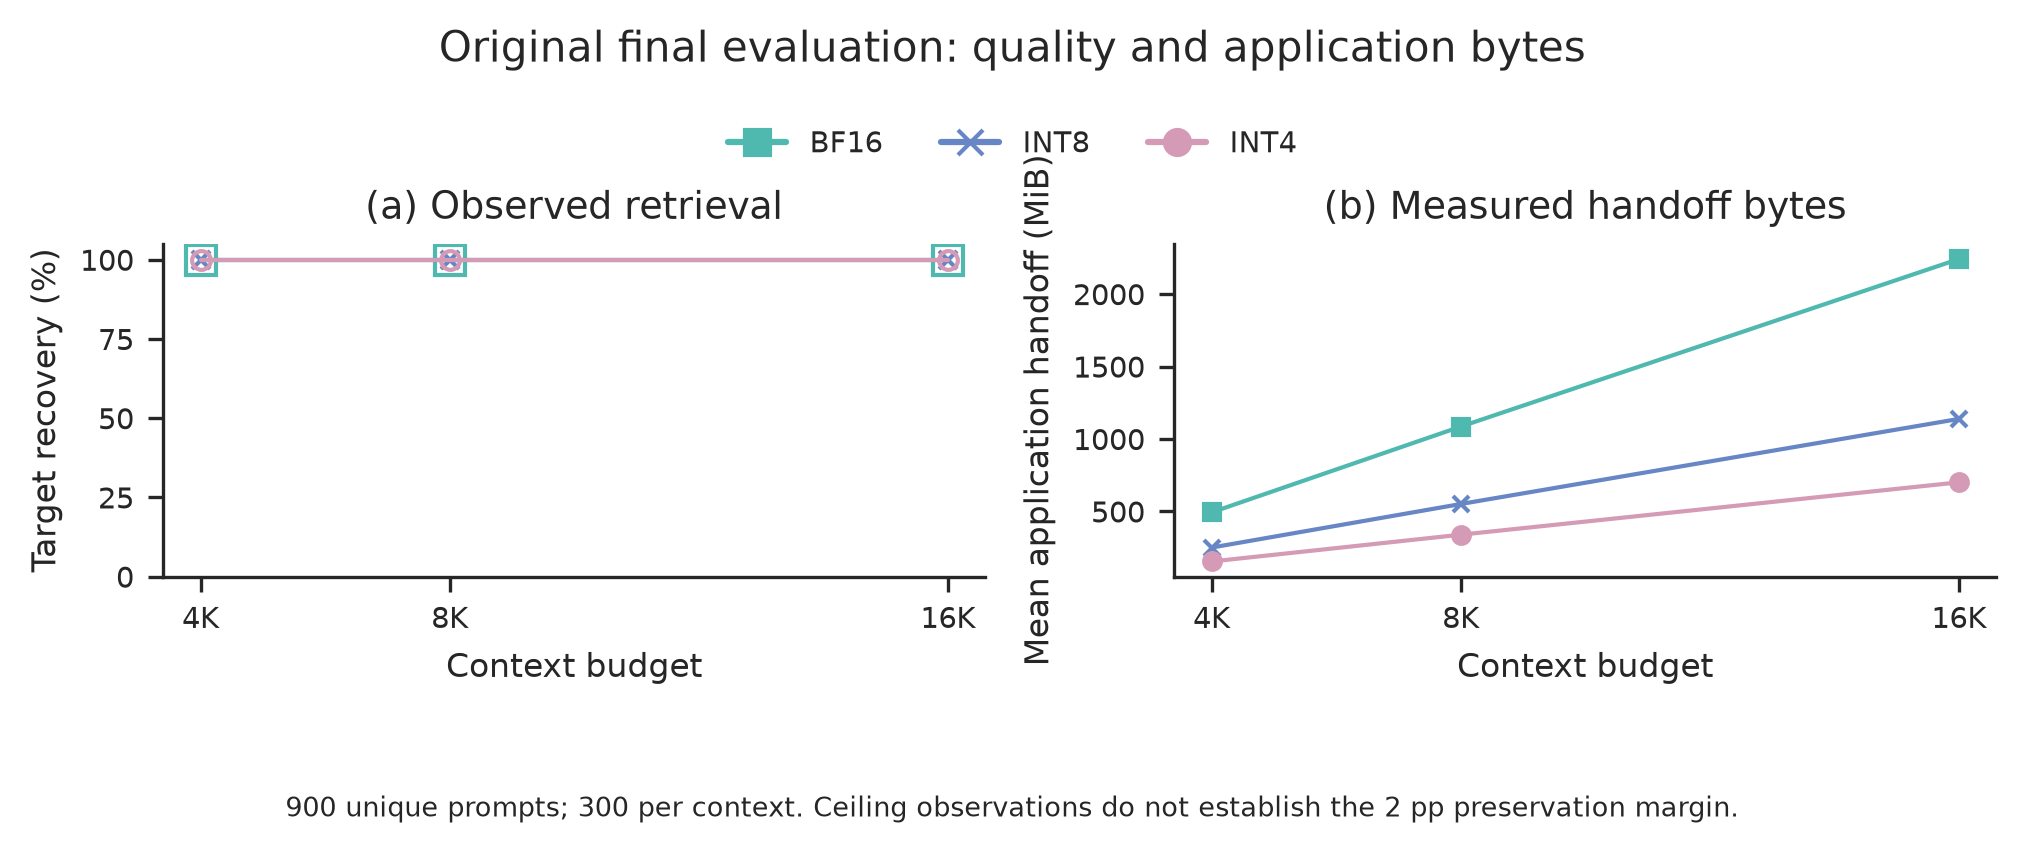
\includegraphics[width=\textwidth]{final-quality-bytes.png}
\caption{Original 900-prompt final evaluation with the PyTorch reference backend. Left:
observed target recovery for native BF16, INT8 and INT4 transfer, with 300 unique
prompts at each context budget (100 per task). All observed scores are at the
ceiling; this does not establish the two-percentage-point preservation margin. Right:
mean application handoff bytes, including payload and counted metadata/control frames
but excluding network headers. Local encoded sizes are not plotted as transmitted
bytes.}
\label{fig:final-quality}
\end{figure*}

\begin{figure*}[t]
\centering
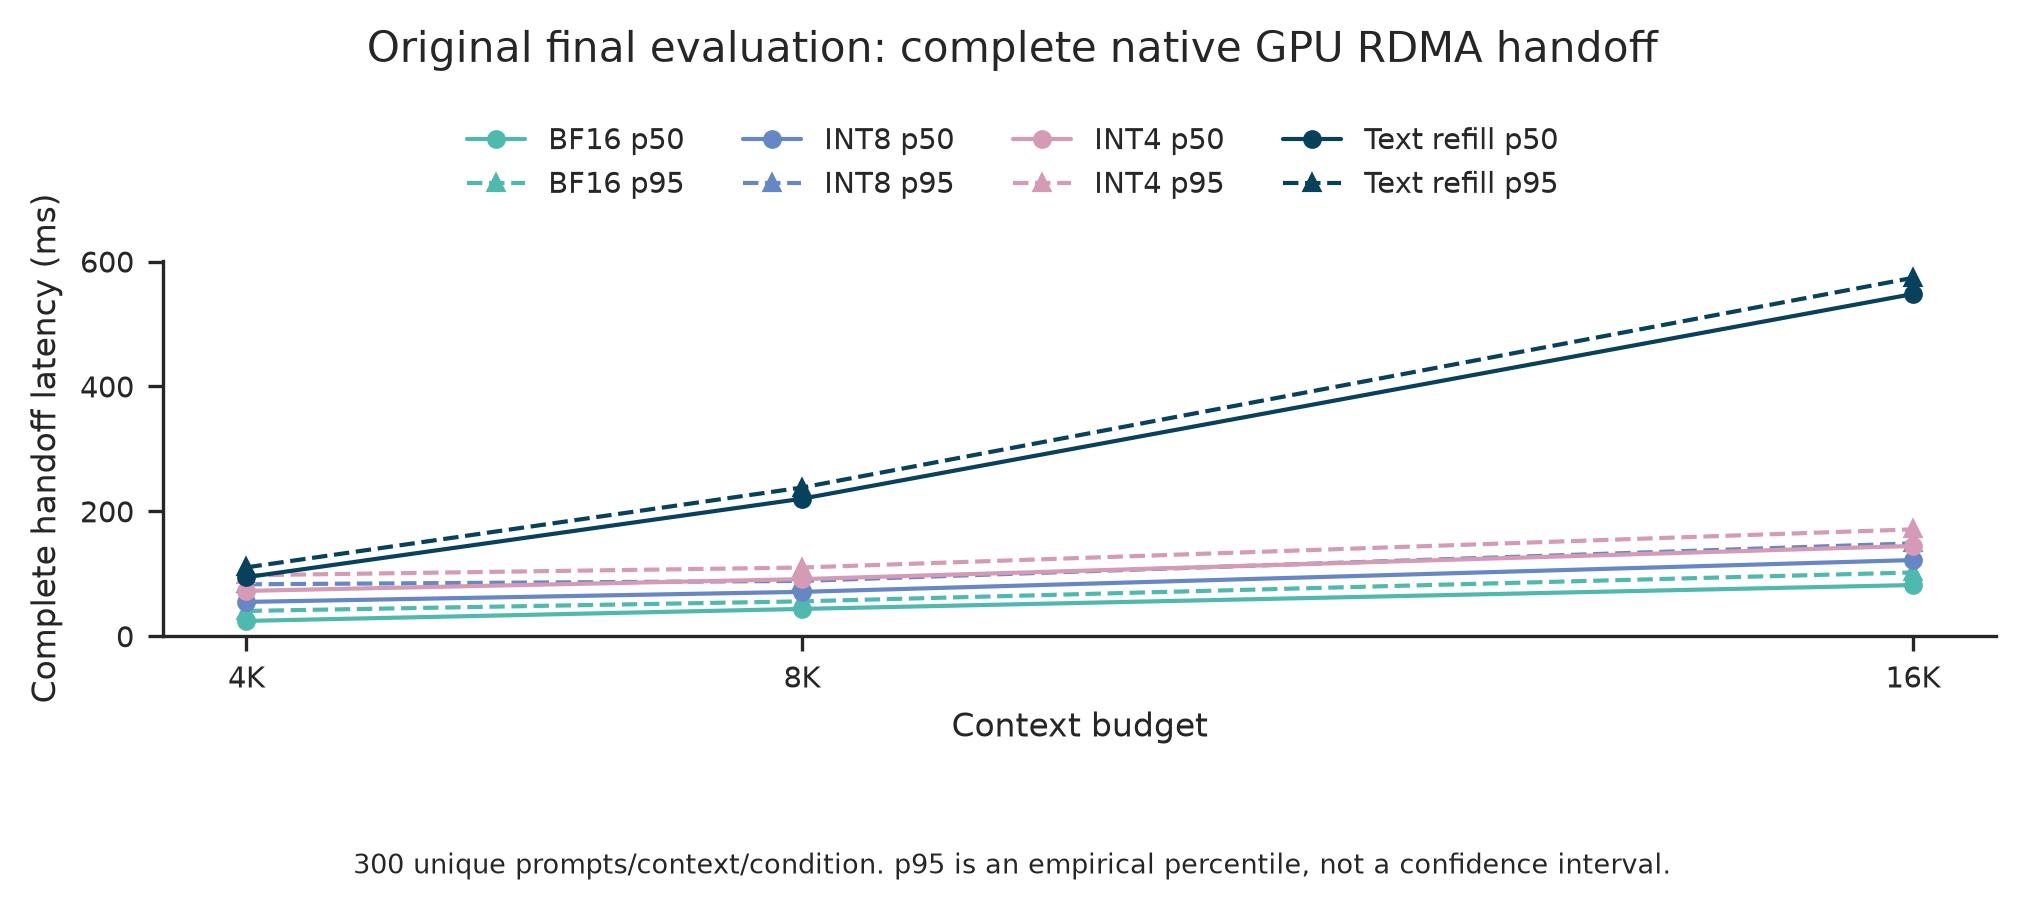
\includegraphics[width=\textwidth]{final-handoff-latency.png}
\caption{Original 900-prompt final evaluation: measured complete native GPU RDMA handoff
latency from sender cache-ready to receiver-ready acknowledgement, including codec,
allocation, registration and control work. Solid lines show medians and dashed lines
show empirical 95th percentiles over 300 unique prompts per context and condition.
These percentiles are descriptive, not confidence intervals. Text refill includes
receiver tokenization and prefill.}
\label{fig:final-latency}
\end{figure*}
\subsection{Original reference study: retained findings}
The original study verified 900 unique final prompts, all 6,300 predictions,
zero execution failures and 3,600 exact local/remote token-ID comparisons.
All seven conditions achieved 100\% target and all-answer recovery in each
task/context cell. Every observed quantized-minus-BF16 score difference was
zero; there were no added or restored targets. The one-sided conservative lower
bound was $-2.95$ percentage points per 100-prompt comparison without
multiplicity adjustment and $-5.72$ points after the within-family adjustment.
The proposed two-point preservation margin therefore remains
\emph{inconclusive}, despite no observed score loss.

In the reference implementation, mean per-prompt application-byte reductions
were 49.22\% for INT8 and 68.71\% for INT4
(Figure~\ref{fig:final-quality}). At the 16K budget, pooled median
BF16/INT8/INT4 handoff latencies were 81.89/121.88/144.51\,ms, versus
547.95\,ms for text refill, with 300 prompts per condition at that budget.
BF16 had the lowest pooled p50 and p95 at every context
(Figure~\ref{fig:final-latency}). Separate original timing blocks supported
the same descriptive ordering. These findings remain valid for the reference
backend; the optional implementation changes neither those measurements nor
their verification record. Full original tables and figures remain available
in the original manuscript and analysis (Appendix~\ref{sec:repro}).



\begin{figure*}[t]
\centering
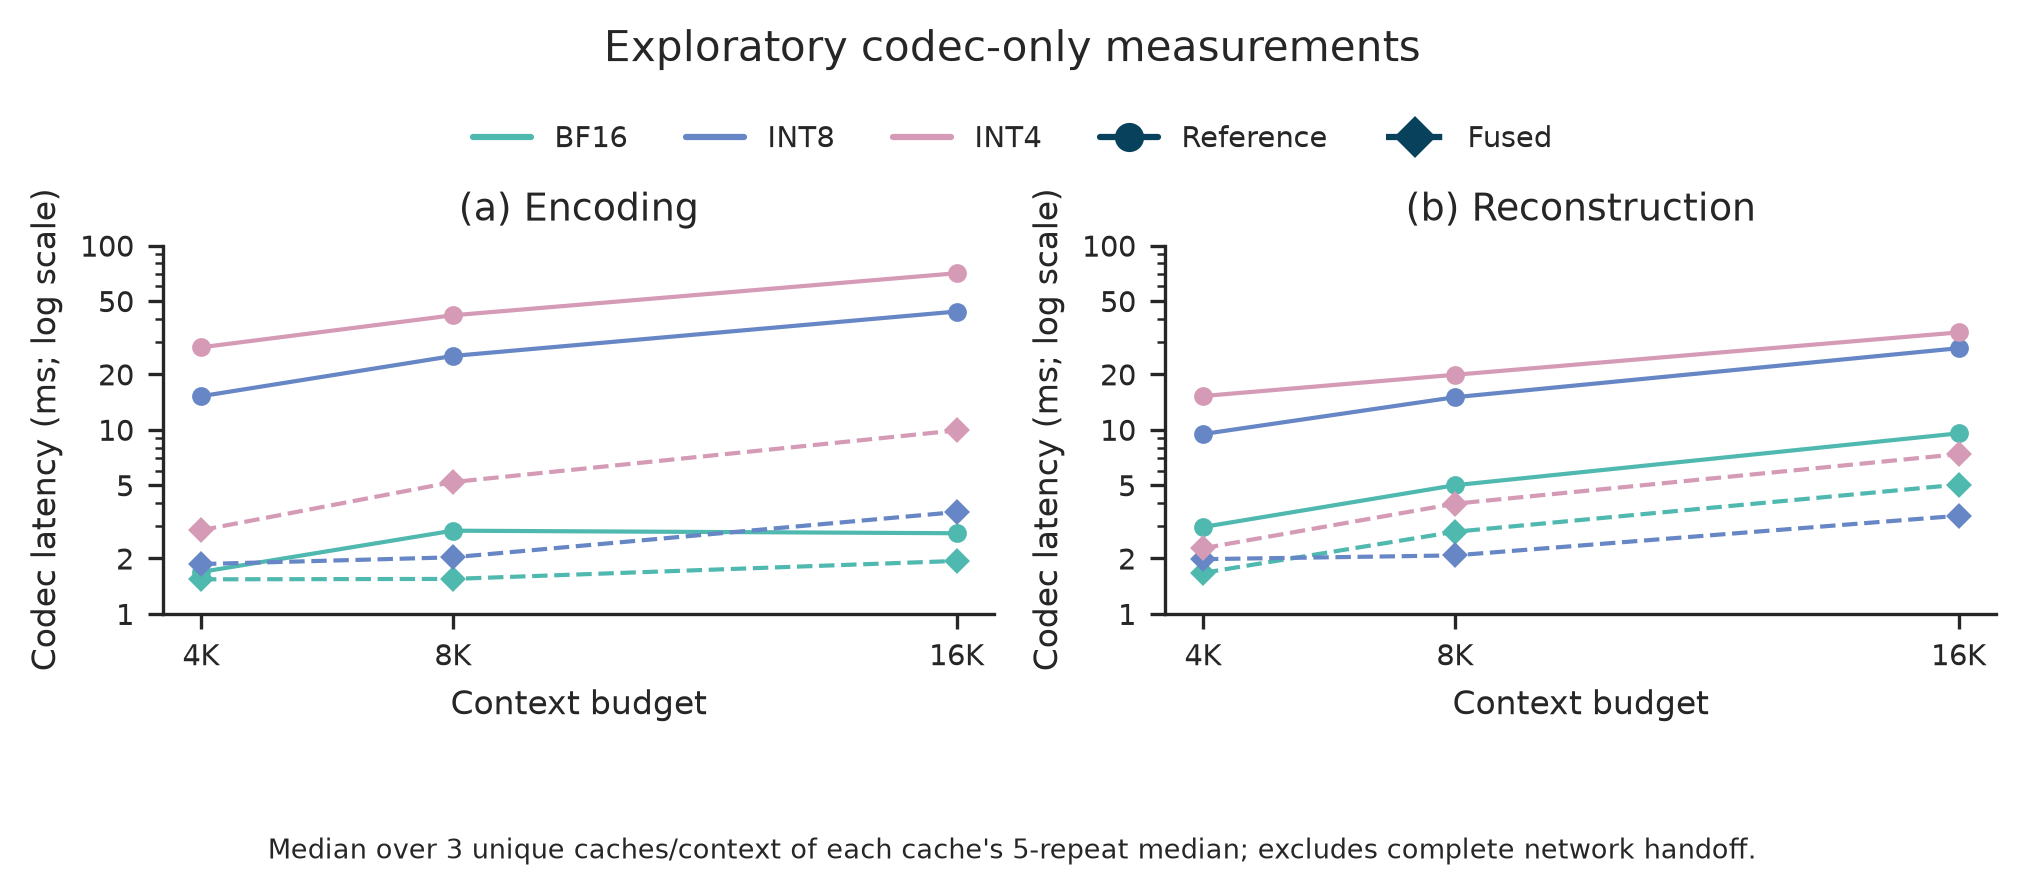
\includegraphics[width=\textwidth]{codec-phase-latency.png}
\caption{Codec-only encode and decode measurements on nine unique real model caches, with five
timed repetitions per cache/backend/precision. Each point is the median across three
prompts at that context of each prompt's five-repeat median. Logarithmic latency axes
make both reference and fused measurements visible. Codec timings exclude complete
network handoff; separately aggregated phase medians need not sum to the
combined-latency median.}
\label{fig:codec}
\end{figure*}

\subsection{Actual-model compatibility and codec-only measurements}
The final performance revision passed all 27 prompt/precision integrity cells
and produced all 54 backend timing rows. The checks compare complete encoded
payloads and canonical headers, all four encoder/decoder combinations, and
reconstructed cache bits; raw BF16 is also checked against the original model
cache. No measured JIT cache misses occurred. These are actual Qwen caches,
not random synthetic tensors. The microbenchmark does not generate predictions.

Table~\ref{tab:codec} reports the median, across three unique prompts per
context, of each prompt's sum of five-repeat encode and decode medians.
These descriptive stage summaries are not complete handoff times and are not
sums of aggregate percentiles (Figure~\ref{fig:codec}). At 16K, INT8 encode
and decode stage medians were 43.85 and 27.73\,ms in the reference, versus
3.57 and 3.41\,ms in the fused backend; INT4 stages were 70.78/33.77 versus
9.92/7.37\,ms. Removing intermediate storage also reduced allocation peaks.
At 16K, median decoded-cache stage peak increments were approximately
4,570\,MiB in the reference and 2,285\,MiB in the fused backend. These include
output-cache residency and are not pure scratch.

\begin{table}[t]
\centering\small
\caption{Codec-only encode-plus-decode summaries (ms). Each row summarizes
three unique prompts, with five repeats per stage/backend/prompt.}
\label{tab:codec}
\setlength{\tabcolsep}{5pt}
\begin{tabular}{llrr}
\toprule Budget & Format & Reference & Fused \\
\midrule
4K & BF16 & 4.67 & 3.21 \\
4K & INT8 & 24.71 & 3.86 \\
4K & INT4 & 43.23 & 5.13 \\
8K & BF16 & 7.82 & 4.34 \\
8K & INT8 & 40.18 & 4.11 \\
8K & INT4 & 61.73 & 9.18 \\
16K & BF16 & 12.30 & 6.98 \\
16K & INT8 & 71.58 & 6.99 \\
16K & INT4 & 104.52 & 17.30 \\
\bottomrule
\end{tabular}
\end{table}


\subsection{Matched native handoff pilot}
All three blocks passed the complete gate: six files, 378 successful
predictions, zero execution failures, 189 exact cross-backend generated-token
comparisons and 216 exact within-backend local/remote comparisons. All target
and all-answer scores were one. These are repeated observations on \emph{nine
unique pilot prompts}, not 378 independent quality examples. Encoded payload
and metadata lengths matched for every cross-backend pair; the separate codec
checks establish actual content equality on the exercised model caches.

Table~\ref{tab:handoff} and Figure~\ref{fig:paired} show complete handoff
measurements. Each context/backend/precision cell contains nine repeated
observations from three unique prompts across three blocks.

\begin{table}[t]
\centering\small
\caption{Matched pilot complete handoff p50/p95 (ms). Nine repeated observations
per row/backend derive from three unique prompts across three blocks.}
\label{tab:handoff}
\setlength{\tabcolsep}{4pt}
\begin{tabular}{llrr}
\toprule Budget & Format & Reference & Fused \\
\midrule
4K & BF16 & 25.08/29.24 & 24.10/30.04 \\
4K & INT8 & 56.22/60.35 & 19.98/32.95 \\
4K & INT4 & 76.17/80.17 & 16.17/17.69 \\
8K & BF16 & 43.87/55.63 & 40.36/50.11 \\
8K & INT8 & 70.94/84.65 & 28.73/47.67 \\
8K & INT4 & 91.32/100.43 & 24.87/26.26 \\
16K & BF16 & 81.46/100.32 & 79.76/95.85 \\
16K & INT8 & 124.11/130.62 & 49.03/55.56 \\
16K & INT4 & 144.28/153.54 & 43.62/47.80 \\
\bottomrule
\end{tabular}
\end{table}

\begin{figure*}[t]
\centering
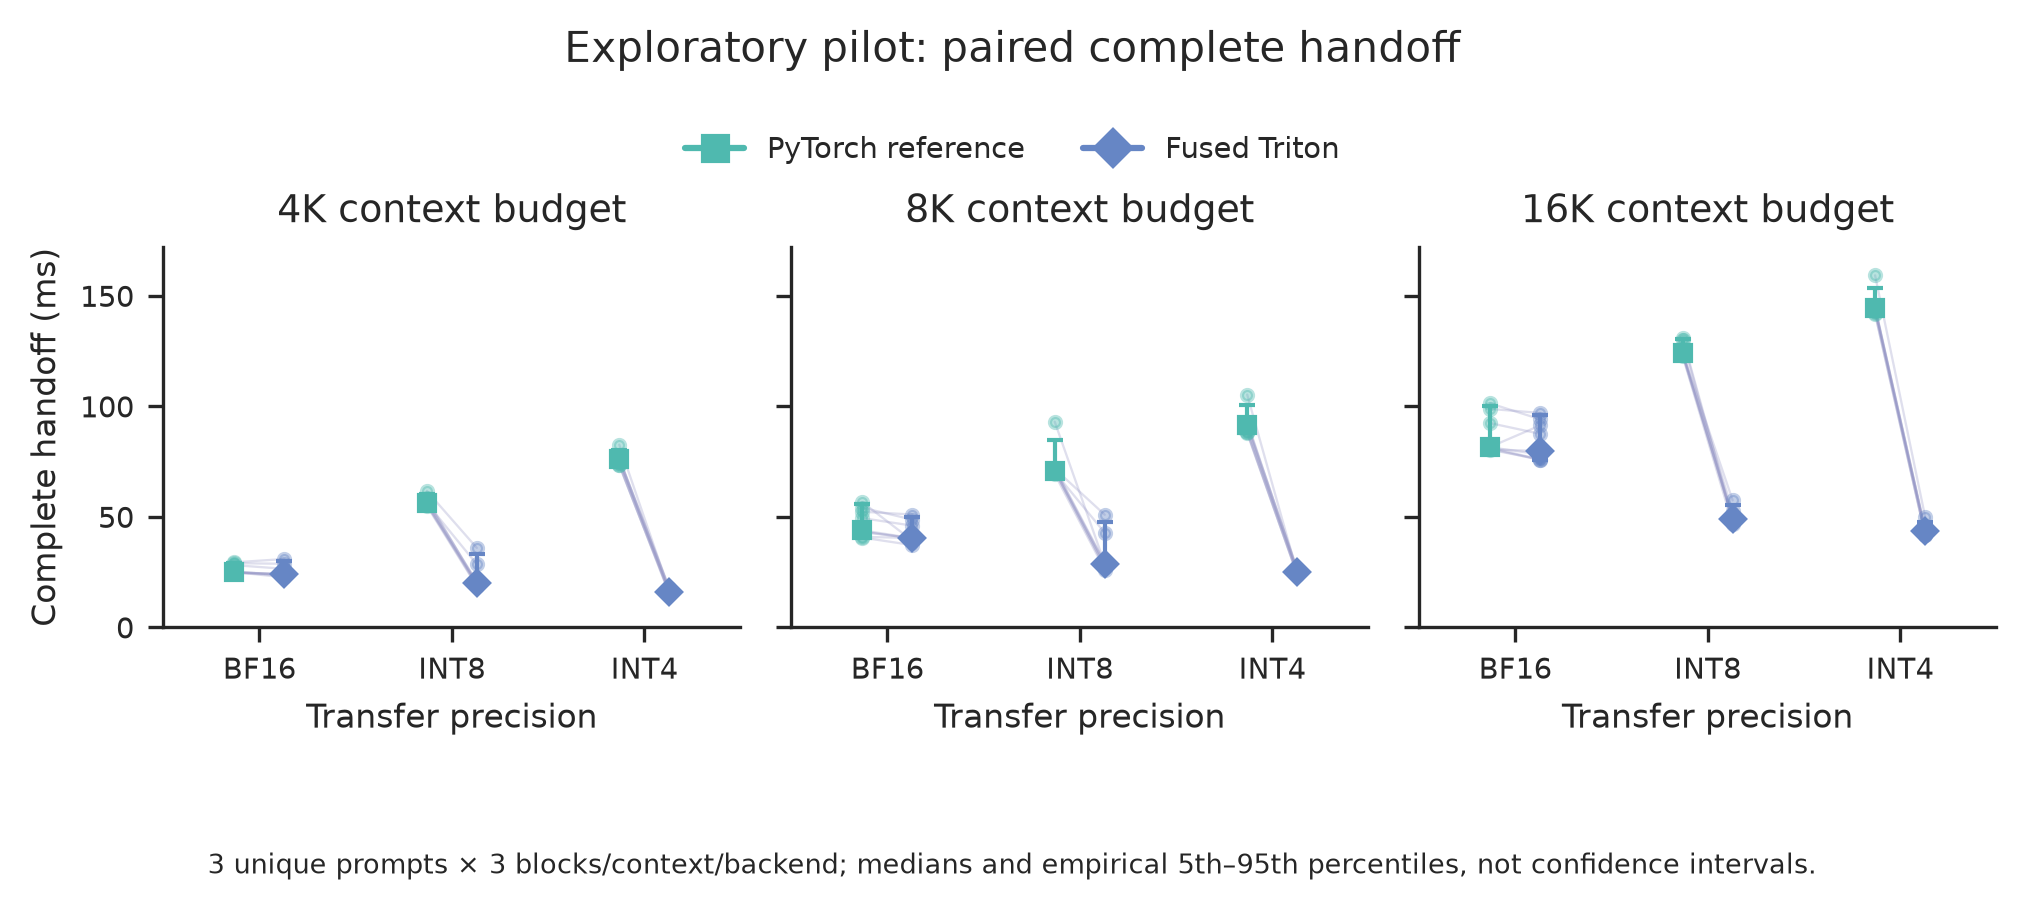
\includegraphics[width=\textwidth]{pilot-paired-handoff.png}
\caption{Exploratory comparison on nine unique pilot prompts repeated in three process blocks.
Thin lines pair the same prompt and block across the reference and fused backends;
each context/backend/precision has nine observations from three unique prompts. Large
markers show medians and whiskers show empirical 5th--95th percentiles, not
confidence intervals. BF16 is optimized in the fused backend too. Blocks 1 and 2
overlapped on disjoint node pairs after block 0 completed; the comparison does not
establish a population speedup.}
\label{fig:paired}
\end{figure*}

Matched ratios are computed per prompt and block before summarization. Median
fused/reference handoff ratios for INT8 were 0.358, 0.396 and 0.392 at
4K/8K/16K; INT4 ratios were 0.215, 0.273 and 0.303. Within the fused backend,
median INT8/BF16 ratios were 0.837, 0.712 and 0.615; INT4/BF16 ratios were
0.657, 0.609 and 0.548 (Figure~\ref{fig:ratios}). Quantized transfer therefore
had lower measured median latency than BF16 in this optional implementation.
INT8 did not uniformly dominate the tail: its within-backend paired p95 ratios
exceeded one at 4K and 8K, and its pooled 4K p95 exceeded fused BF16. INT4 had
lower pooled p50 and p95 than fused BF16 at all three contexts in this pilot.

\begin{table}[t]
\centering\small
\caption{Ranges of block-specific median fused/reference handoff ratios.
These ranges describe three process blocks, not confidence intervals.}
\label{tab:blocks}
\setlength{\tabcolsep}{5pt}
\begin{tabular}{lrr}
\toprule Budget & INT8 range & INT4 range \\
\midrule
4K & 0.341--0.360 & 0.207--0.215 \\
8K & 0.387--0.610 & 0.273--0.276 \\
16K & 0.391--0.398 & 0.302--0.307 \\
\bottomrule
\end{tabular}
\end{table}

Table~\ref{tab:blocks} retains block variation. Block 0 ran alone; blocks 1/2
overlapped on disjoint node pairs. Variation cannot be attributed solely to
implementation or treated as independent hardware replication. Text-refill
medians changed little between backends: 110.12/110.69, 236.47/238.02 and
572.51/574.95\,ms for reference/fused at the three contexts. This baseline is
reported rather than assumed invariant.

\begin{figure*}[t]
\centering
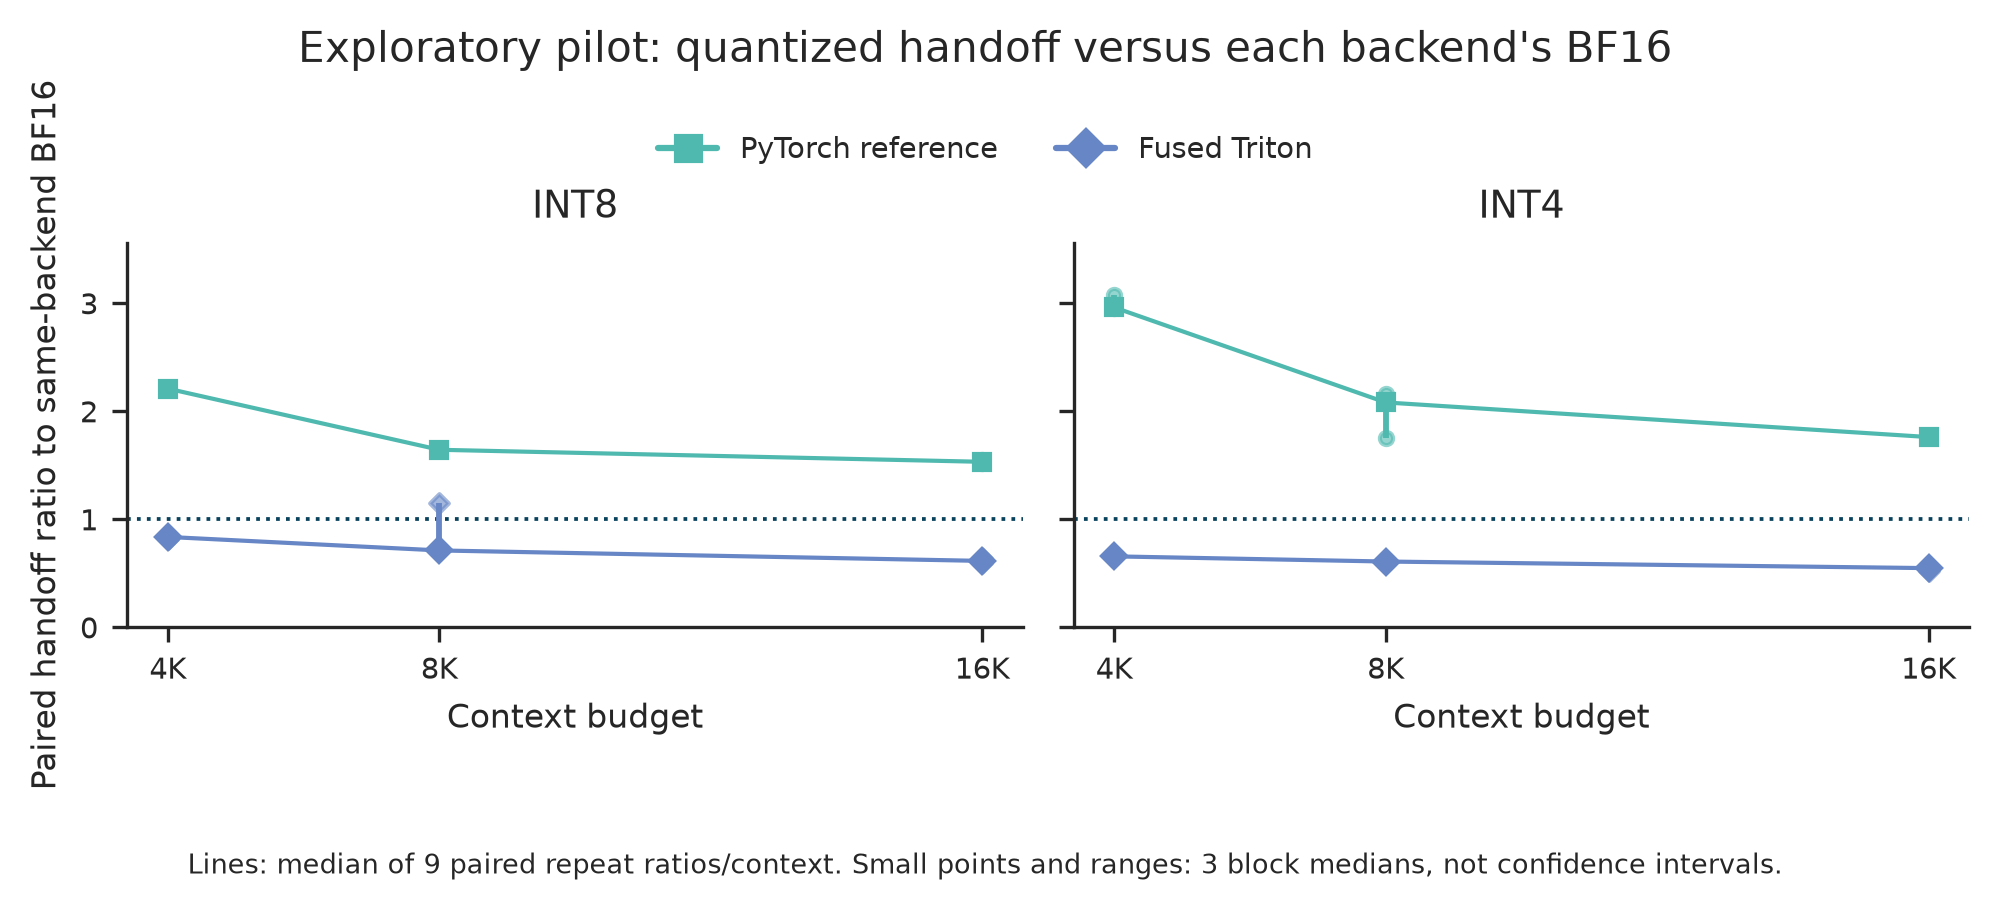
\includegraphics[width=\textwidth]{pilot-paired-bf16-ratios.png}
\caption{Exploratory same-backend comparison: INT8 or INT4 complete handoff divided by BF16
complete handoff for the same prompt and block. Lines show the median of nine paired
ratios at each context (three unique prompts repeated in three blocks); vertical
ranges span the three block medians, which are also shown as small points. Values
below one indicate lower measured latency in this pilot. Ranges are descriptive, not
confidence intervals; scheduling and node-placement variation remain possible.}
\label{fig:ratios}
\end{figure*}

\begin{table}[t]
\centering\small
\caption{16K pilot median sender/receiver handoff allocation increments (MiB).
Both columns include reconstructed-cache residency where applicable.}
\label{tab:memory}
\setlength{\tabcolsep}{3pt}
\begin{tabular}{lrr}
\toprule Format & Reference S/R & Fused S/R \\
\midrule
BF16 & 4,578.77/6,892.88 & 2,284.88/4,589.70 \\
INT8 & 2,320.58/5,768.29 & 1,160.29/3,465.12 \\
INT4 & 1,429.18/5,322.20 & 714.20/3,019.03 \\
\bottomrule
\end{tabular}
\end{table}

Table~\ref{tab:memory} and Figure~\ref{fig:memory} report handoff allocation
increments. They include frame and reconstructed-cache residency, using each
worker's measured handoff baseline. They exclude later continuation cloning/
generation and unobserved non-PyTorch allocations, and differ from the
codec-only stage increments above.

\begin{figure*}[t]
\centering
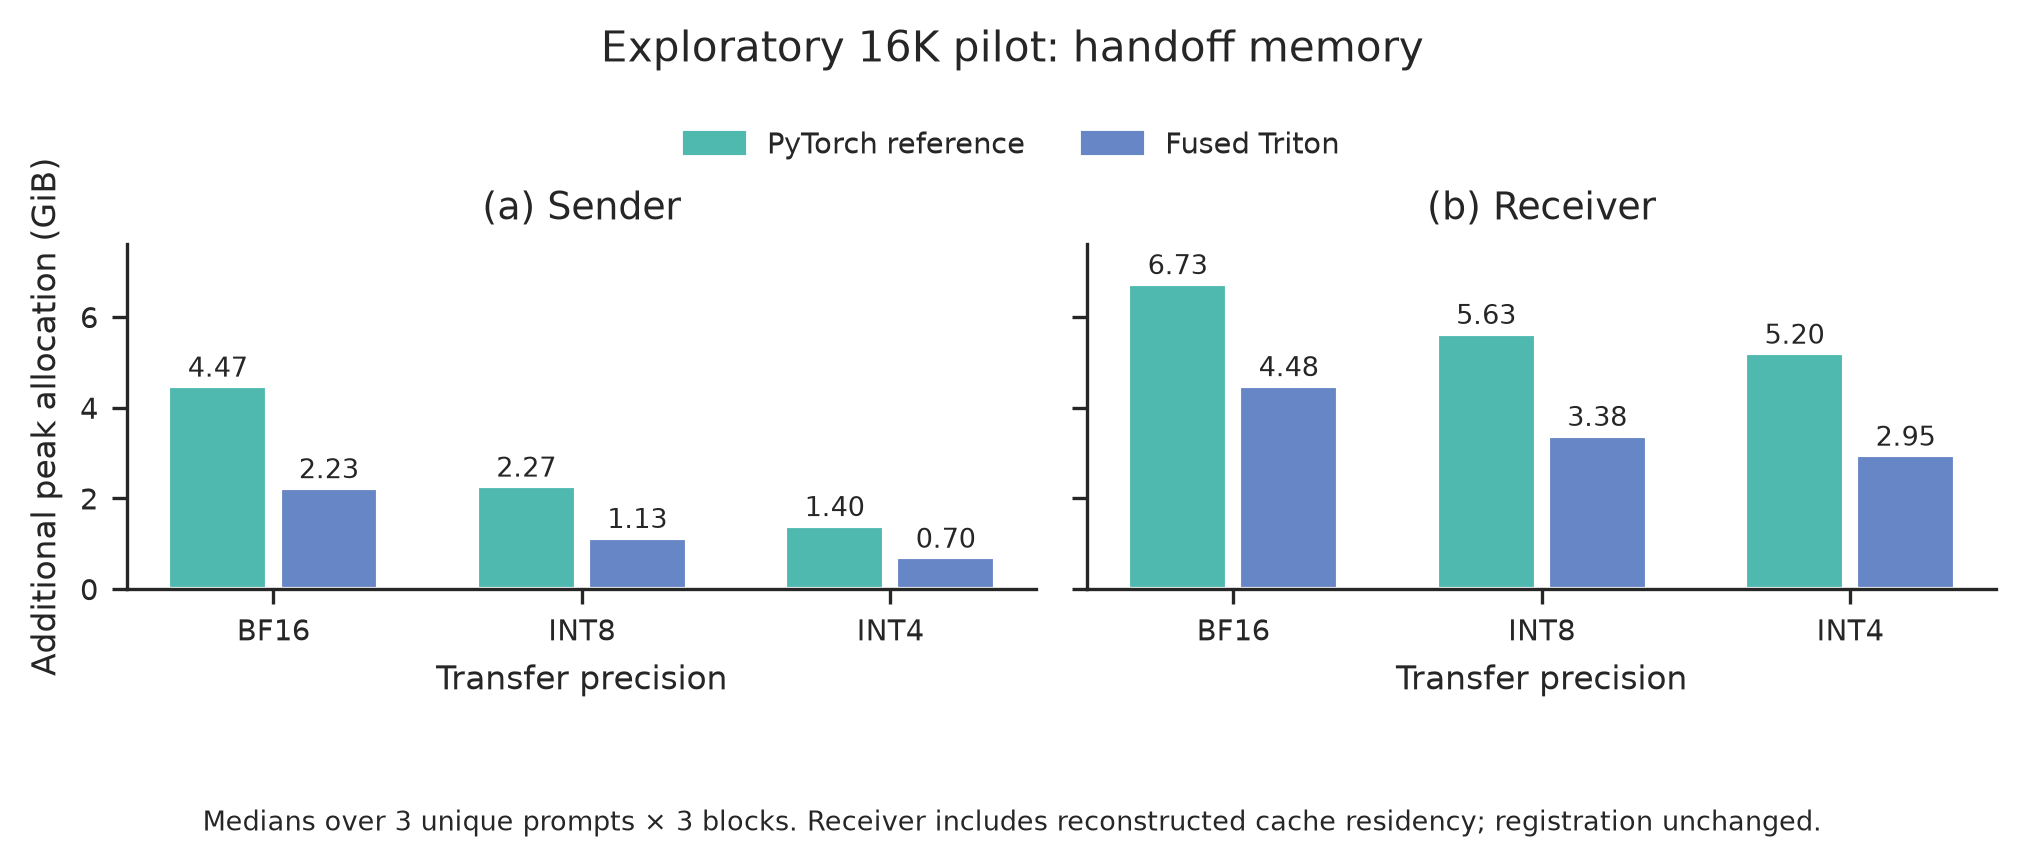
\includegraphics[width=\textwidth]{pilot-handoff-memory.png}
\caption{Exploratory 16K pilot handoff memory: median additional peak allocation above the
sender's or receiver's measured handoff baseline, for three unique prompts repeated
in three blocks. Receiver values include reconstructed BF16 cache residency, not only
temporary codec workspace. Per-request registration remains unchanged. Bars are
descriptive medians and are not confidence bounds.}
\label{fig:memory}
\end{figure*}

\section{Discussion and limitations}
The original study established that fewer bytes did not yield faster complete
handoff with its reference implementation. The optional backend tests a more
specific explanation: allocation, packing and cache-construction costs are
implementation-dependent contributors to that interval. Codec-only measurements
support a substantial reduction in these stages while preserving encoded
contents and reconstructed cache bits. The paired native pilot also shows that
these reductions can change the observed precision ordering: fused INT8/INT4
had lower median complete handoff than fused BF16 at every tested context,
whereas quantization increased the reference backend's median. This supports
an implementation-specific revision of the latency conclusion, without
invalidating the original measurements or extending the pilot result to the
full retrieval population. The comparison includes direct cache adoption as
well as fused kernels, so it does not identify each optimization's causal effect.

The new performance evidence is a nine-prompt pilot, repeated in three blocks.
It is not a second 900-prompt quality trial. Matching bytes and outputs on
exercised inputs supports implementation compatibility, but does not prove
universal numerical equivalence, population noninferiority or production
serving performance. Shared nodes, overlapping block schedules, differing node
pairs and a small repeated prompt set limit generalization. Block ranges and
empirical percentiles are descriptive, not confidence intervals.

The first output token remains sender-selected; only subsequent tokens attend
to reconstructed cache. Target-substring recovery does not fully measure
fluency, unsupported text or reasoning. The three synthetic retrieval tasks and
one model create ceiling effects and sparse losses. Correlated targets and
repeated prompts cannot supply additional independent quality evidence. The
original conservative two-point-margin conclusion remains inconclusive.

Both backends retain sequential encoding, transport and reconstruction with
registration per handoff/request. Neither experiment measures a pipelined,
adaptive, multi-request or constrained-link serving system. A fully optimized
production codec, different fabric or registration policy could change the
remaining cost balance; no such result is inferred here.

\FloatBarrier
\appendix
\section{Reproducibility and version boundaries}\label{sec:repro}
This versioned manuscript combines the original reference study with a
separate optional-backend experiment. The original manuscript, original
900-prompt study and its 111 verified artifacts remain unchanged. The source
pins are as follows; long identifiers are retained here rather than in the
main experimental narrative.

\paragraph{Pinned inputs and formats.}
\begin{itemize}\setlength{\itemsep}{2pt}
\item Model: {\small\nolinkurl{Qwen/Qwen3-4B-Instruct-2507}}, revision
{\small\nolinkurl{cdbee75f17c01a7cc42f958dc650907174af0554}}.
\item RULER revision:
{\small\nolinkurl{db43f92ff634bbce1c33d1fb15858aec4bba509a}}.
\item Packed format: {\small\nolinkurl{bonsai-torch-packed-v1}}.
\item Explicit backends: {\small\nolinkurl{pytorch_packed_v1}} and
{\small\nolinkurl{triton_packed_v1}}. The transport binding is
{\small\nolinkurl{FabricEndpoint}}.
\end{itemize}

\paragraph{Original and new artifacts.}
The original artifacts remain at
{\small\nolinkurl{runs/final-20261107}} and
{\small\nolinkurl{results/analysis-final}}; the original manuscript is
{\small\nolinkurl{docs/PAPER_DRAFT.md}}. The new frozen source, copied inputs,
submission record, codec measurements and paired results are under
{\small\nolinkurl{runs/fused-20261108}}. The original detailed campaign tables
are {\small\nolinkurl{results/analysis-final/campaign/campaign.md}}.

Performance snapshot v2 uses this SHA256 for
{\small\nolinkurl{bench/bonsai_bench/fused.py}}:
\par\noindent{\small\nolinkurl{8c865a7b9fbb0c2b56b57d779983cdf8786f7ec8de6e961ba6b604d2788a593c}}.
It is shared by the actual-model microbenchmark and paired performance
snapshot. The scheduling change is retained in
{\small\nolinkurl{runs/fused-20261108/submission.json}}.

The exact codec aggregation and integrity records are
{\small\nolinkurl{runs/fused-20261108/codec/aggregate.json}} and
{\small\nolinkurl{runs/fused-20261108/codec/summary.json}}. Paired measurements,
block tables and provenance are
{\small\nolinkurl{runs/fused-20261108/analysis/summary.md}} and
{\small\nolinkurl{runs/fused-20261108/analysis/summary.json}}. The original paired
pilot PNG remains at
{\small\nolinkurl{runs/fused-20261108/analysis/paired-handoff.png}}; this article
uses PNG figures prepared from the same measured artifacts.

\paragraph{Tests and postfreeze changes.}
The measured revision passed 43 real-H200 codec tests before the performance
run. A later live alignment-hardening revision passed 61 H200 tests in job
1306126. The later live CPU suite passed 132 tests, with 60 GPU-only cases
skipped there. These later tests are separate robustness evidence; they do not
change the frozen code or reported performance. Postfreeze alignment handling
must not be credited with measured speedups.

\paragraph{Integrity and reproduction.}
The paired analysis checks actual frozen benchmark hashes, every sidecar's
source map, the audited pilot-file bytes and all nine canonical prompt hashes.
All six result files must pass failure, completeness, ownership-sensitive
continuation and cross-backend checks before reporting. Postprocessing sources
are archived separately from the immutable runtime snapshot. Output paths are
restricted to the new run, including symlink resolution, to protect the
original artifacts. Full packet contents are checked by the codec integrity
benchmark; diagnostic hashing is outside timing.

Implementation and reproduction commands are documented in
{\small\nolinkurl{docs/FUSED_CODEC.md}}; original statistical definitions are in
{\small\nolinkurl{docs/ANALYSIS.md}}. All figure exports are PNG. The reference
manuscript remains the record of the original complete study; this revision
records the optional implementation experiment and its narrower scope.

\bibliographystyle{unsrt}
\bibliography{references}
\end{document}
